\renewcommand*{\arraystretch}{1.1}

\noindent\begin{tabularx}{17cm}{|>{\small \sf}c|X|}
	\hline
	query    & Interactive / complex / 6 \\ \hline
%
	title       & Tag co-occurrence \\ \hline
%
    pattern     & \hfill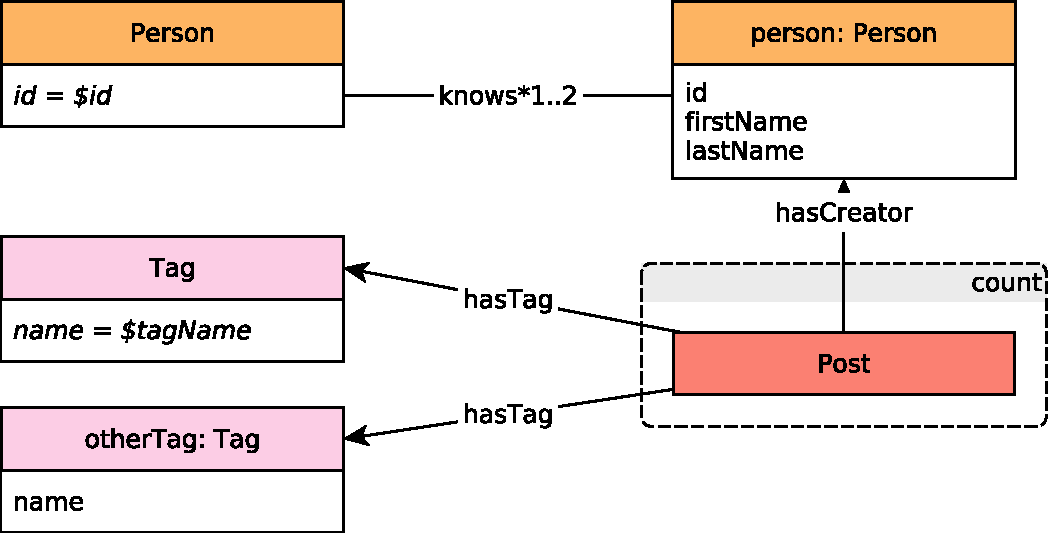
\includegraphics[scale=\patternscale,margin=0cm .2cm]{patterns/interactive-complex-read-06}\hfill\vadjust{} \\ \hline
%
	desc. & Given a start Person and some Tag, find the other Tags that occur
together with this Tag on Posts that were created by start Person's
friends and friends of friends (excluding start Person). Return For each
Tag, find the count of Posts that were created by these Persons, which
contain both this Tag and the given Tag.
 \\ \hline
%
	
%
	params.  &
	\vspace{1.1ex}{\begin{tabularx}{14.66cm}{|c|M|m{2cm}|Y|} \hline
	\cellcolor{parameter} \color{white} $\mathsf{1}$ & \varname{Person.id} & \cellcolor{gray!20} \vartype{ID} &  \\ \hline
	\cellcolor{parameter} \color{white} $\mathsf{2}$ & \varname{Tag.name} & \cellcolor{gray!20} \vartype{String} &  \\ \hline
	\end{tabularx}}\vspace{1.1ex} \\ \hline
%
	
	result      &
	\vspace{1.1ex}{\begin{tabularx}{14.66cm}{|c|M|m{2cm}|c|Y|} \hline
	\cellcolor{result} \color{white} $\mathsf{1}$ & \varname{Tag.name} & \cellcolor{gray!20} \vartype{String} &
	    \texttt{R} &
	     \\ \hline
	\cellcolor{result} \color{white} $\mathsf{2}$ & \varname{count} & \cellcolor{gray!20} \vartype{32-bit Integer} &
	    \texttt{A} &
	    number of Posts that were created by friends and friends of friends, which contain this Tag \\ \hline
	\end{tabularx}}\vspace{1.1ex} \\ \hline
	
%
	sort        &
	\vspace{1.1ex}{\begin{tabular}{|c|l|c|} \hline
	\cellcolor{sort} \color{white} $\mathsf{1}$ & \varname{count} & \cellcolor{gray!20} $\desc$ \\ \hline
	\cellcolor{sort} \color{white} $\mathsf{2}$ & \varname{Tag.name} & \cellcolor{gray!20} $\asc$ \\ \hline
	\end{tabular}}\vspace{1.1ex} \\ \hline
	%
	limit       & 10 \\ \hline
	%
	CPs &
	\multicolumn{1}{>{\raggedright}l|}{
	  \chokepoint{5.1}
	  } \\ \hline
	%
    relevance &
      \small This query looks for paths of lengths three or four, starting from a Given Person, moving to friends or friends of
friends, then to Posts and finally ending at a given Tag.
 \\ \hline%
\end{tabularx}
\vspace{2ex}